
\documentclass[11pt,a4paper,twoside]{article}

% ----------------------------------------------------------------------
% Define external packages, language, margins, fonts and new commands
% ----------------------------------------------------------------------
%\input{preamble} 
\usepackage[utf8]{inputenc}
\usepackage[english]{babel} 
\usepackage{notoccite}
\usepackage[skip=0.5\baselineskip]{caption}
\hyphenation{GTKWave}
\usepackage{listings}
\usepackage[all]{nowidow}


\usepackage{graphicx}
\graphicspath{{./}{../../figlib/}{../mat/}{../sim/}}
\def\FontLn{% 16 pt normal
  \usefont{T1}{phv}{m}{n}\fontsize{16pt}{16pt}\selectfont}
\def\FontLb{% 16 pt bold
  \usefont{T1}{phv}{b}{n}\fontsize{16pt}{16pt}\selectfont}
\def\FontMn{% 14 pt normal
  \usefont{T1}{phv}{m}{n}\fontsize{14pt}{14pt}\selectfont}
\def\FontMb{% 14 pt bold
  \usefont{T1}{phv}{b}{n}\fontsize{14pt}{14pt}\selectfont}
\def\FontSn{% 12 pt normal
  \usefont{T1}{phv}{m}{n}\fontsize{12pt}{12pt}\selectfont}

%Use Arial font as default
%
\renewcommand{\rmdefault}{phv}
\renewcommand{\sfdefault}{phv}
\usepackage{geometry}	
\geometry{verbose,tmargin=2.5cm,bmargin=2.5cm,lmargin=2.5cm,rmargin=2.5cm}

%\usepackage{setspace}
%\renewcommand{\baselinestretch}{1.5}

\usepackage[pdftex]{hyperref} % enhance documents that are to be
                              % output as HTML and PDF
\hypersetup{colorlinks,       % color text of links and anchors,
                              % eliminates borders around links
%            linkcolor=red,    % color for normal internal links
            linkcolor=black,  % color for normal internal links
            anchorcolor=black,% color for anchor text
%            citecolor=green,  % color for bibliographical citations
            citecolor=black,  % color for bibliographical citations
%            filecolor=magenta,% color for URLs which open local files
            filecolor=black,  % color for URLs which open local files
%            menucolor=red,    % color for Acrobat menu items
            menucolor=black,  % color for Acrobat menu items
%            pagecolor=red,    % color for links to other pages
            pagecolor=black,  % color for links to other pages
%            urlcolor=cyan,    % color for linked URLs
            urlcolor=black,   % color for linked URLs
	          bookmarks=true,         % create PDF bookmarks
	          bookmarksopen=false,    % don't expand bookmarks
	          bookmarksnumbered=true, % number bookmarks
	          pdftitle={report},
            pdfauthor={Andre C. Marta},
%            pdfsubject={Thesis Title},
%            pdfkeywords={Thesis Keywords},
            pdfstartview=FitV,
            pdfdisplaydoctitle=true}

\usepackage[numbers,sort&compress]{natbib} % <<<<< References in numbered list [1],[2],...
\usepackage{subcaption} 
\usepackage{mdframed}

%%%%%%%%%%%%%%%%%%%%%%%%%%%%%%%%%%%%%%%%%%%%%%%%%%%%%%%%%%%%%%%%%%%%%%%%
%     Begin Document                                                   %
%%%%%%%%%%%%%%%%%%%%%%%%%%%%%%%%%%%%%%%%%%%%%%%%%%%%%%%%%%%%%%%%%%%%%%%%


\begin{document}


\pagestyle{plain}


\thispagestyle {empty}

% IST Logo - Signature A
% parameters: bb=llx lly urx ury (bounding box), width=h_length, height=v_length, angle=angle, scale=factor, clip=true/false, draft=true/false. 
\includegraphics[bb=9.5cm 11cm 0cm 0cm,scale=0.29]{IST_A_CMYK_POS}

\begin{center}
%
% Figure (Image or plot)
\vspace{1.0cm}
% height = 50 mm
%\includegraphics[height=50mm]{Figures/Airbus_A350.jpg}



% Title, author and degree
\vspace{1cm}
{\FontLb Circuit Theory and Electronics Fundamentals} \\ 
\vspace{1cm}
{\FontSn Integrated Master in Aerospace Engineering, Técnico, University of Lisbon} \\ 
\vspace{1cm}
{\FontSn Laboratory Report-T3} \\
\vspace{1cm}
{\FontSn May 5th, 2021} \\ 
\vspace{1cm}
{\FontSn António Cordeiro 95769} \\ 
\vspace{00.5cm}
{\FontSn Catarina Falcão 95775} \\ 
\vspace{0.5cm}
{\FontSn Luís Pinheiro 97230} \\ 
\end{center}

\newpage





% ----------------------------------------------------------------------
%  Table of contents, list of tables, list of figures and nomenclature
% ----------------------------------------------------------------------

% Table of contents
%
\tableofcontents

\newpage

% List of tables
%\addcontentsline{toc}{section}{\listtablename}
%\listoftables
%\cleardoublepage 

% List of figures
%\addcontentsline{toc}{section}{\listfigurename}
%\listoffigures
%\cleardoublepage 

% Set arabic numbering (1,2,...) after preface
%
%\setcounter{page}{1}
%\pagenumbering{arabic}

% ----------------------------------------------------------------------
%  Body
% ----------------------------------------------------------------------

\section{Introduction}
\label{sec:introduction}


The main objective of this laboratory assignment is to analyse a circuit using a simulation and the node and mesh methods. It is important to rely on a method that simplifies a circuit as it gives us many information. So, it is equally important to understand if these methods can be applied and if the results are satisfactory. To prove the truthfulness of this analysis, the following report was developed. The circuit can be seen in Figure~\ref{fig:circuit}.

In the next section (~\ref{sec:analysis}), we briefly explain the procedure to analyse the given circuit, first with the node method and then with the mesh method. In order to solve the necessary calculations and obtain the values for the tension and current in every node and branch, respectively, we used Octave maths tool.
Then, we resorted to Ngspice to simulate our circuit and obtain the simulated values for the same physical quantities previously calculated. These values will be shown in Section~\ref{sec:simulation}. We will also compare both results and give certain notes related to our analysis.
The report finishes with its conclusion, in section~\ref{sec:conclusion}, where we resume the most important points of the lab assignment.


\begin{figure}[h] \centering
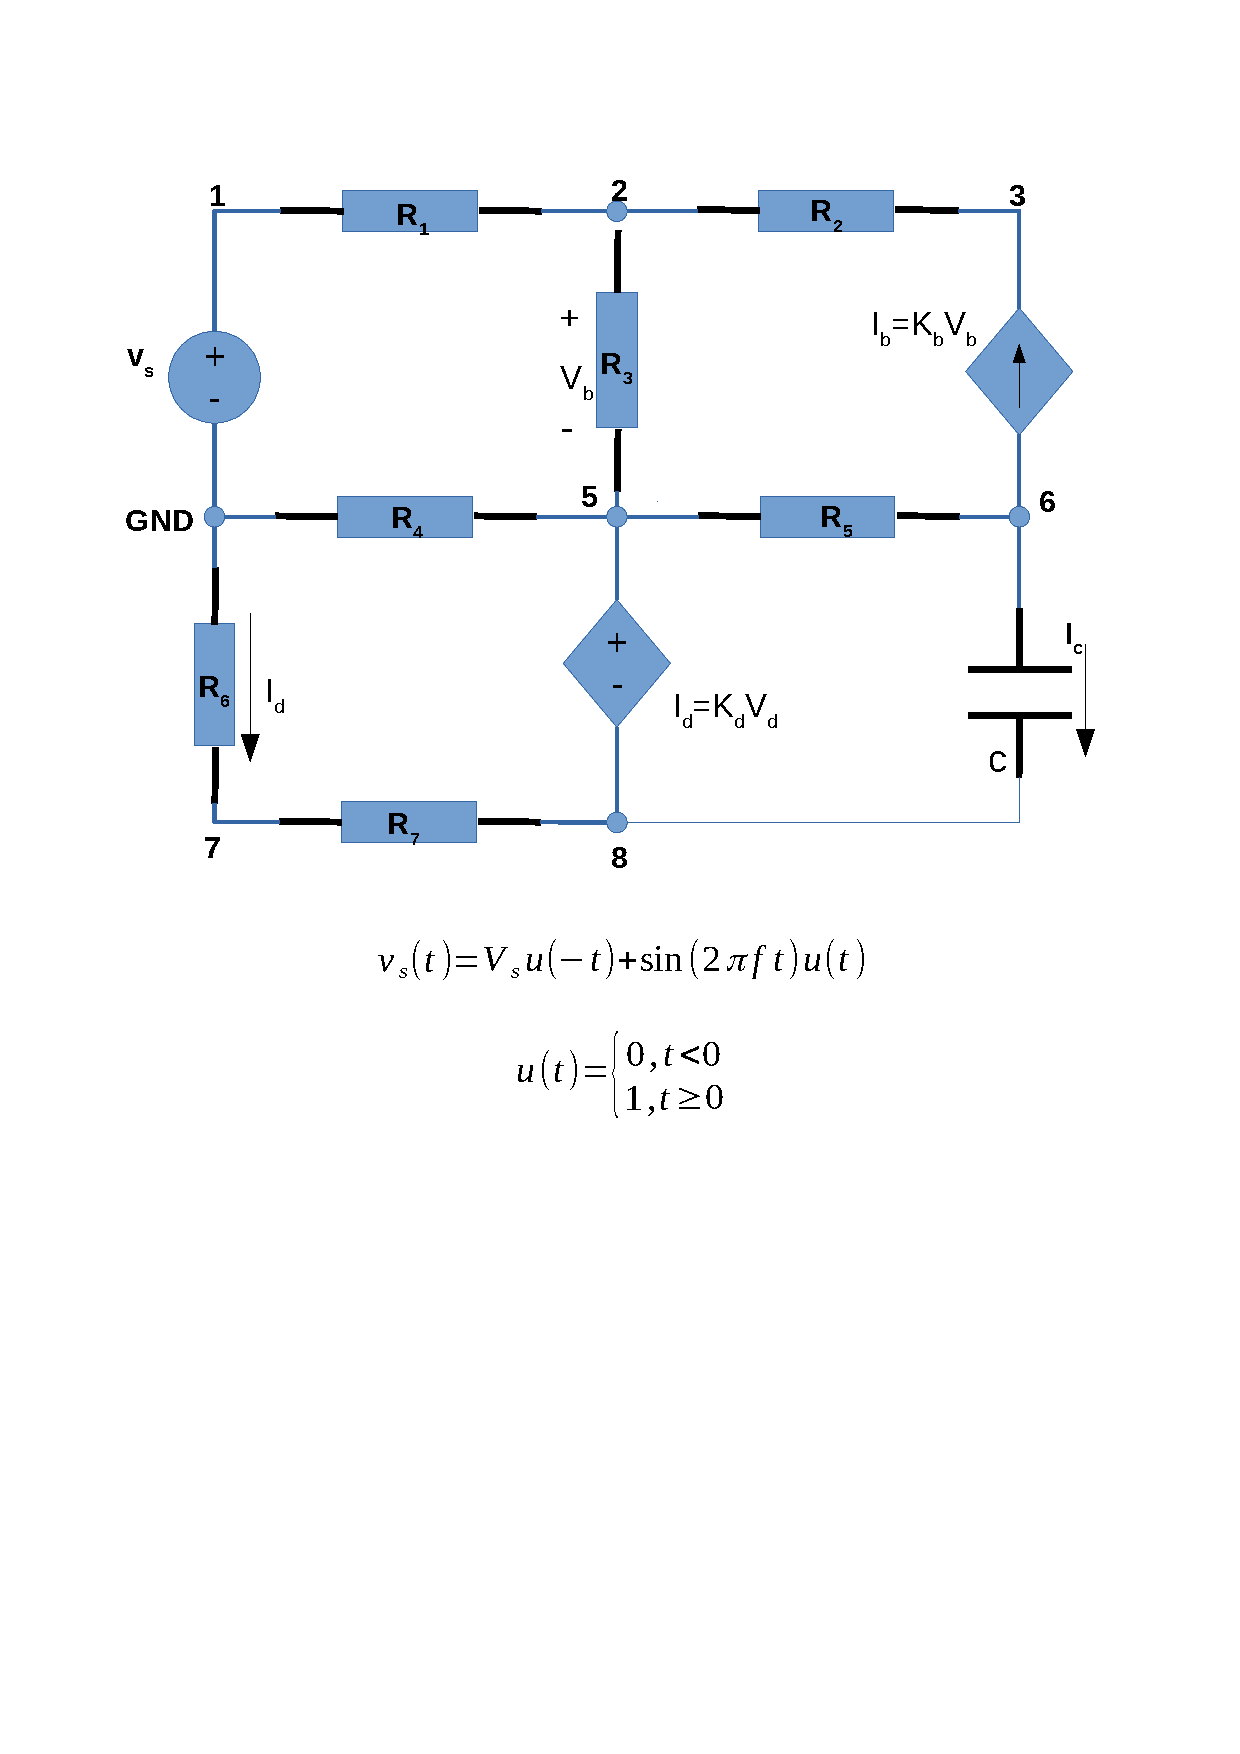
\includegraphics[width=0.6\linewidth]{circuit.pdf}
\caption{Circuit under analysis.}
\label{fig:circuit}
\end{figure}







\section{Theoretical Analysis}
\label{sec:analysis}

In this section, the circuit shown in Figure~\ref{fig:rc} is analysed
theoretically, in terms of its time and frequency responses.

\section{Time response}

The circuit consists of a single V-R-C loop where a current $i(t)$ circulates. The
voltage source $v_I(t)$ drives its input, and the output voltage $v_O(t)$ is taken from
the capacitor terminals. Applying the Kirchhoff Voltage Law (KVL), a single
equation for the single loop in the circuit can be written as

\begin{equation}
  Ri(t) + v_O(t) = v_I(t).
  \label{eq:kvl}
\end{equation}

Because $v_O$ is the voltage between capacitor C's plates, it is related to the
current $i$ by
\begin{equation}
  i(t) = C\frac{dv_O}{dt}.
\end{equation}

Hence, Equation~(\ref{eq:kvl}) can be rewritten as
\begin{equation}
  RC\frac{dv_O}{dt} + v_O(t) = v_I.
  \label{eq:kvl2}
\end{equation}

Equation~(\ref{eq:kvl2}) is a linear differencial equation whose solution is a
superposition of a natural solution $v_{On}$ and a forced solution $v_{Of}$:

\begin{equation}
  v_O(t) = v_{On}(t) + v_{Of}(t).
  \label{eq:vo_sol}
\end{equation}

As learned in the theory classes the natural solution is of the form
\begin{equation}
  v_{On}(t) = Ae^{-\frac{t}{RC}}.
  \label{eq:vo_nat}
\end{equation}
where $A$ is an integration constant.

The forced solution is of the form given in Equation~(\ref{eq:vo_for}) and is
illustrated in Figure~\ref{fig:forced}.

\begin{equation}
  V_{Of}(t) = |\bar{V}_{Of}| cos(\omega t + \angle \bar{V}_{Of}),
  \label{eq:vo_for}
\end{equation}

\lipsum[1-1]


\begin{figure}[h] \centering
\includegraphics[width=0.8\linewidth]{forced.eps}
\caption{Forced sinusoidal response.}
\label{fig:forced}
\end{figure}

\section{Frequency response}

\lipsum[1-1]




\section{Simulation Analysis}
\label{sec:simulation}

\subsection{Operating Point Analysis}

Table~\ref{tab:op} shows the simulated operating point results for the circuit
under analysis. Compared to the theoretical analysis results, one notices the
following differences: describe and explain the differences.

\begin{table}[h]
  \centering
  \begin{tabular}{|l|r|}
    \hline    
    {\bf Name} & {\bf Value [A or V]} \\ \hline
    \input{../sim/op_tab}
  \end{tabular}
  \caption{Operating point. A variable preceded by @ is of type {\em current}
    and expressed in Ampere; other variables are of type {\it voltage} and expressed in
    Volt.}
  \label{tab:op}
\end{table}

\lipsum[1-1]


\subsection{Transient Analysis}

Figure~\ref{fig:trans} shows the simulated transient analysis results for the
circuit under analysis. Compared to the theoretical analysis results, one
notices the following differences: describe and explain the differences.

\begin{figure}[h] \centering
\includegraphics[width=0.6\linewidth]{trans.eps}
\caption{Transient output voltage}
\label{fig:trans}
\end{figure}

\lipsum[1-1]



\subsection{Frequency Analysis}

\subsubsection{Magnitude Response}

Figure~\ref{fig:acm} shows the magnitude of the frequency response for the
circuit under analysis. Compared to the theoretical analysis results, one
notices the following differences: describe and explain the differences.

\begin{figure}[h] \centering
\includegraphics[width=0.6\linewidth]{acm.eps}
\caption{Magnitude response}
\label{fig:acm}
\end{figure}

\lipsum[1-1]

\subsubsection{Phase Response}

Figure~\ref{fig:acp} shows the magnitude of the frequency response for the
circuit under analysis. Compared to the theoretical analysis results, one
notices the following differences: describe and explain the differences.

\begin{figure}[h] \centering
\includegraphics[width=0.6\linewidth]{acp.eps}
\caption{Phase response}
\label{fig:acp}
\end{figure}

\lipsum[1-1]

\subsubsection{Input Impedance}

Figure~\ref{fig:zim} shows the magnitude of the frequency response for the
circuit under analysis. Compared to the theoretical analysis results, one
notices the following differences: describe and explain the differences.

\begin{figure}[h] \centering
\includegraphics[width=0.6\linewidth]{zim.eps}
\caption{Input impedance}
\label{fig:zim}
\end{figure}

\lipsum[1-1]





\section{Conclusion}
\label{sec:conclusion}

In this laboratory assignment, the objective of analysing a circuit was achieved. Theoretical calculations were made using both mesh and node methods. Then, a simulation of the given circuit was produced and the results were perfectly similar to the previously calculated values.
One reason for these satisfactory results is the fact that this circuit containes only linear components and so it was expected that the results would not differ.
In resume, the reliability of these methods was proven, since we obtained relative errors with a maximum order of magnitude equal to (-4). Since the results were very precise, one deduces the methods can be used in order to help analysing circuits.

%\cleardoublepage


\end{document}
